\subsection{Fluid-Structure Interaction between an elastic object and laminar incompressible flow} \label{sec:HronTurek}
The goal of this benchmark is to verify the fluid and solid solver first separately and then together as a full FSI problem \cite{Hron2006a}. This benchmark is based on the older benchmark " flow around cylinder" with fluid considered incompressible and in the laminar regime where the structure deformations are large, in one case the deformations are about 2.5 larger than the height of the elastic object. The problem is setup with the solid submerged in the fluid, so that oscillations in the fluid can deform the structure. Measuring the drag and lift around the circle and bar, and measure structural displacement at a given point. This benchmark will be used to test and verify different numerical methods and code implementations. Testing the robustness and efficiency of the FSI implementation


\subsection*{Problem Defintion}
\subsubsection*{Domain}

\begin{center}
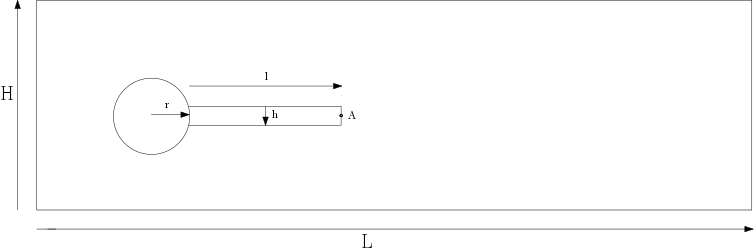
\includegraphics[scale=0.4]{./Verification_Validation/Hron_Turek/Domain_drawing.png}
\end{center}

The computational domain consists of a circle with an elastic bar behind the circle. The circle is positioned at (0.2, 0.2) making it 0.05 of center from bottom to top, \textbf{this shift in the domain is done to induce oscillations to an otherwise steady flow}. The fluid oscillations gives a force to the elastic bar. The parameters of the domain are:\\
L = 2.5, H = 0.41, l = 0.35, h = 0.02, A = (0.2, 0.6) \\

\subsubsection*{Boundary conditions}
A parabolic profile has been prescribed to the velocity that increases over time until a time = 2 has been reached.

\begin{align*}
u(0,y) &= 1.5u_0 \frac{y(H-y)}{(\frac{H}{2})^2}  \\
u(0,y,t) &= u(0,y)\frac{1-cos(\frac{\pi}{2}t)}{2} \text{  for  } t<2.0 \\
u(0,y,t) &= u(0,y) \text{  for  } t \leq 2.0
\end{align*}

Setting no slip on the "floor" and "ceiling" so to speak.\\
$$ u(x,y,t) = 0 \text{  on  } \partial \mathcal{F}_{floor and ceiling} $$
$$  p(x,y,t) = 0 \text{  on  } \partial \mathcal{F}_{outlet} $$

\subsubsection*{Quantities for comparison}
When the fluid moves around the circle and bar it exerts a force. These are split into drag and lift and calculated as follows:
$$ (F_d, F_L) = \int_S \sigma_f n dS $$ 
where S is the part of the circle and bar in contact with the fluid. \\
We set a point $A = (0.2,0.6)$ on the right side of the bar. This point is used to track the deformation. \\
In the unsteady time dependent problems, the values are represented by mean and amplitude values:
\begin{align}
mean =& \frac{1}{2} (max + min) \\
amplitude =& \frac{1}{2} (max - min)\\
\end{align}

In each test the numbers with ref are the values taken from the original benchmark paper \cite{Hron2006a}

\subsubsection{Results}
\subsubsection{CFD test}
The first two CFD tests are run with Reynolds numbers 20 and 100 converging to steady solutions of drag and lift around the circle. The CFD 3 problem has a Reynolds number 200 which will induce oscillations behind the circle, giving fluctuations in the drag and lift, hence giving unsteady solutions.
The CFD tests can be run in two ways. The first way assumes the bar to be rigid object, meaning that the computing domain is just the fluid domain. The other way, which is implemented here, is running the full FSI code and setting $\rho_s=10^{6}$ and $\mu_s=10^{12}$, so that the bar is almost completely rigid, only giving rise to very small deformation (in the $10^{-9}$ range).

\begin{figure}[H]
\caption{Fluid mesh}
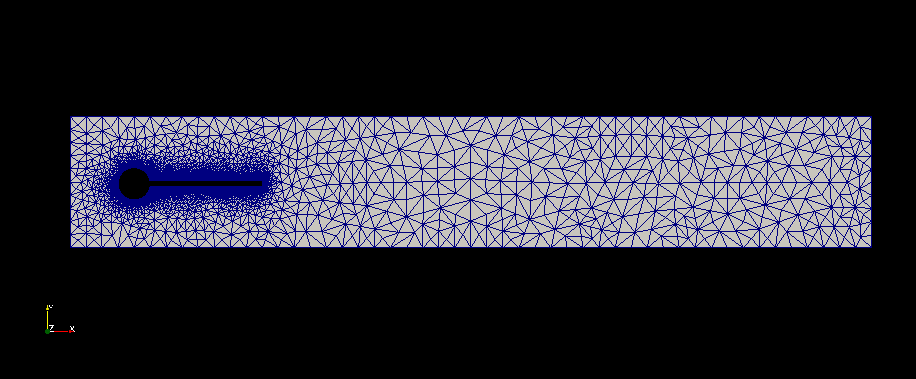
\includegraphics[scale=0.5,trim={24mm 46mm 14mm 40mm},clip]{./Verification_Validation/Hron_Turek/fluid.png}
\end{figure}

\vspace{1cm}

\begin{table}[H]
\centering
\caption{Summary of all the parameters in CFD tests}
\label{my-label}
\begin{tabular}{|l|l|l|l|}
\hline
Parameters & CFD1 & CFD2 & CFD3 \\ \hline
$\rho_f [10^3 \frac{kg}{m^3}]$ & 1 & 1 & 1 \\ \hline
$\nu_f [10^{-3} \frac{m^2}{s}]$ & 1 & 1 & 1 \\ \hline
$ U [\frac{m}{s}] $ & 0.2 & 1 & 2 \\ \hline
Re = $\frac{Ud}{\nu_f}$ & 20 & 100 & 200 \\ \hline
\end{tabular}
\end{table}

\begin{table}[H]
\centering
\caption{CFD 1}
\label{my-label}
\begin{tabular}{|l|l|l|l|}
\hline
\textbf{elements} & \textbf{dofs} & \textbf{Drag} & \textbf{Lift} \\ \hline
6616 & 32472 & 14.2439 & 1.0869 \\ \hline
26464 & 124488 & 14.2646 & 1.11085 \\ \hline
105856 & 487152 & 14.2755 & 1.11795 \\ \hline
\textbf{ref} & \textbf{} & \textbf{14.29} & \textbf{1.119} \\ \hline
\end{tabular}
\end{table}

\begin{table}[H]
\centering
\caption{CFD 2 with }
\label{my-label}
\begin{tabular}{|l|l|l|l|}
\hline
\textbf{elements} & \textbf{dofs} & \textbf{Drag} & \textbf{Lift} \\ \hline
6616 & 32472 & 135.465 & 6.27158 \\ \hline
26464 & 124488 & 136.566 & 9.82166 \\ \hline
105856 & 487152 & 136.573 & 10.4441 \\ \hline
\textbf{ref} & \textbf{} & \textbf{136.7} & \textbf{10.53} \\ \hline
\end{tabular}
\end{table}

\begin{table}[]
\centering
\caption{CFD 3 with $\Delta t = 0.001$}
\label{my-label}
\begin{tabular}{|l|l|l|l|}
\hline
\textbf{elements} & \textbf{dofs} & \textbf{Drag} & \textbf{Lift} \\ \hline
6616 & 32472 & $ -10.42 \pm 446.57  $ & $ 435.13 \pm 5.02 $ \\ \hline
26464 & 124488 & $ -18.42 \pm 445.57 $ & $ 440.73 \pm 5.22 $ \\ \hline
ref & ref & $\bold{ -11.893 \pm 437.81 }$ & $\bold{ 439.45 \pm 5.61 }$ \\ \hline
\end{tabular}
\end{table}

\subsubsection{CSM test}
The CSM test are calculated using only the bar and adding a gravity term $g$ with the same value but changing the parameters of solid. The tests CSM1 and CSM2 are steady state solutions. The difference is a more slender bar. The CSM 3 test is unsteady and even more slender causing the bar to move up and down. Since there is no resistance from any fluid the unsteady test should if energy is preserved make the bar move up and down infinitely. 

Our quantity for comparing there will be the deformation at the point $A$. 
\begin{center}
\begin{figure}[H]
\caption{Picture of the coarsest solid mesh used in the MMS test}
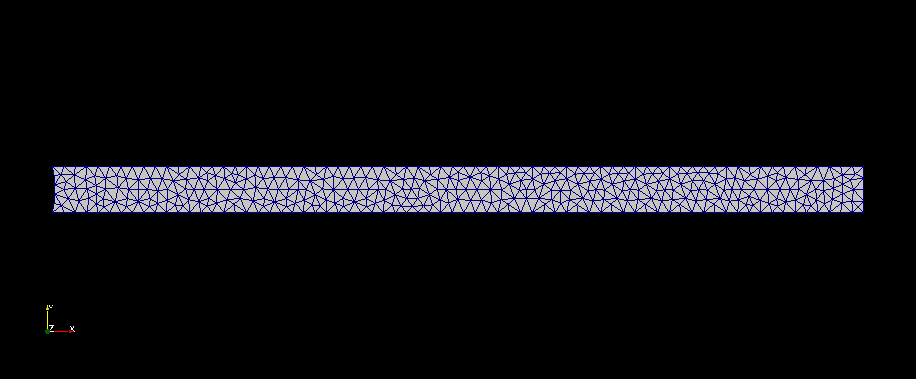
\includegraphics[scale=0.50,trim={18mm 55mm 18mm 55mm},clip]{./Verification_Validation/Hron_Turek/structure.png}
\end{figure}
\end{center}

\vspace{0cm}

\begin{table}[H]
\centering
\caption{Summary table of the parameters used in the CSM tests}
\label{my-label}
\begin{tabular}{|l|l|l|l|}
\hline
Parameters & CSM1 & CSM2 & CSM3 \\ \hline
$\rho_f[10^3 \frac{kg}{m^3}]$ & 1 & 1 & 1 \\ \hline
$\nu_f [10^{-3} \frac{m^2}{s}]$ & 1 & 1 & 1 \\ \hline
$u_0$ & 0 & 0 & 0 \\ \hline
$\rho_s[10^3 \frac{kg}{m^3}]$ & 1 & 1 & 1 \\ \hline
$\nu_s$ & 0.4 & 0.4 & 0.4 \\ \hline
$\mu_s[10^6 \frac{m^2}{s}]$ & 0.5 & 2.0 & 0.5 \\ \hline
$g $ & 2 & 2 & 2 \\ \hline
\end{tabular}
\end{table}

\begin{table}[H]
\centering
\caption{Results of the steady CSM1 case from coarse to fine mesh.}
\label{tab:CSM1}
\begin{tabular}{|l|l|l|l|}
\hline
elements & dofs & $d_x(A) [\times10^{-3}]$ & $d_y(A) [\times10^{-3}]$ \\ \hline
725 & 1756 & -5.809 & -59.47 \\ \hline
2900 & 6408 & -6.779 & -64.21 \\ \hline
11600 & 24412 & -7.085 & -65.63 \\ \hline
46400 & 95220 & -7.116 & -65.74 \\ \hline
\textbf{ref} & \textbf{ref} & \textbf{-7.187} &  \textbf{-66.10} \\ \hline
\end{tabular}
\end{table}

\begin{table}[H]
\centering
\caption{Results of the steady CSM2 case from coarse to fine mesh.}
\label{tab:CSM2}
\begin{tabular}{@{}|l|l|l|l|@{}}
\hline
Elements & Dofs & $d_x(A) [\times10^{-3}] $& $d_y(A) [\times10^{-3}] $\\ \hline
725 &  1756 & -0.375 & -15.19 \\ \hline
2900 & 6408 & -0.441 & -16.46\\ \hline
11600 & 24412 & -0.462 & -16.84 \\ \hline
46400 & 95220 & -0.464 & -16.87\\ \hline
\textbf{ref} & \textbf{ref} &  \textbf{-0.469} &  \textbf{-16.97} \\ \hline
\end{tabular}
\end{table}

\begin{table}[H]
\centering
\caption{Results of the unsteady CSM3 case with mesh from coarse to fine.}
\label{tab:CSM3}
\begin{tabular}{|l|l|l|l|}
\hline
elements & dofs & $d_x(A) [\times10^{-3}]$ & $d_y(A)[\times10^{-3}]$ \\ \hline
725 & 1756 & $-11.743 \pm 11.744$ & $-57.952 \pm 58.940$ \\ \hline
2900 & 6408 & $-13.558 \pm 13.559$ & $ -61.968 \pm  63.440 $ \\ \hline
11600 & 24412 & $ -14.128 \pm 14.127$ & $-63.216 \pm 64.744 $ \\ \hline
46400 & 95220 & $ -14.182 \pm 14.181 $ & $ -63.305 \pm 64.843 $ \\ \hline
\textbf{ref} &  & $ \textbf{-14.305} \pm \textbf{14.305} $ & $ \textbf{-63.607} \pm  \textbf{65.160} $ \\ \hline
\end{tabular}
\end{table}

\begin{figure}[H]  \label{plot:CSM3_plots} 
\centering
  \caption {Results for CSM3 showing Displacement of point A}
  \begin{minipage}[b]{0.60\linewidth}
    \centering
    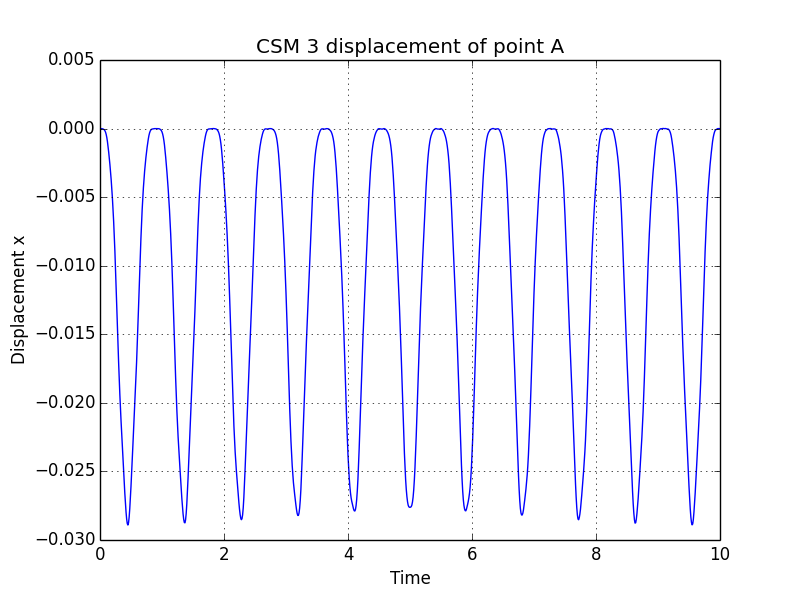
\includegraphics[width=0.9\linewidth,trim={2mm 2mm 5mm 5mm},clip]{./Verification_Validation//Hron_Turek/dis_x.png} 
    \caption{Displacement in x direction, timeinterval (0,10)} 
    \vspace{4ex}
  \end{minipage}%%
  \begin{minipage}[b]{0.60\linewidth}
    \centering
    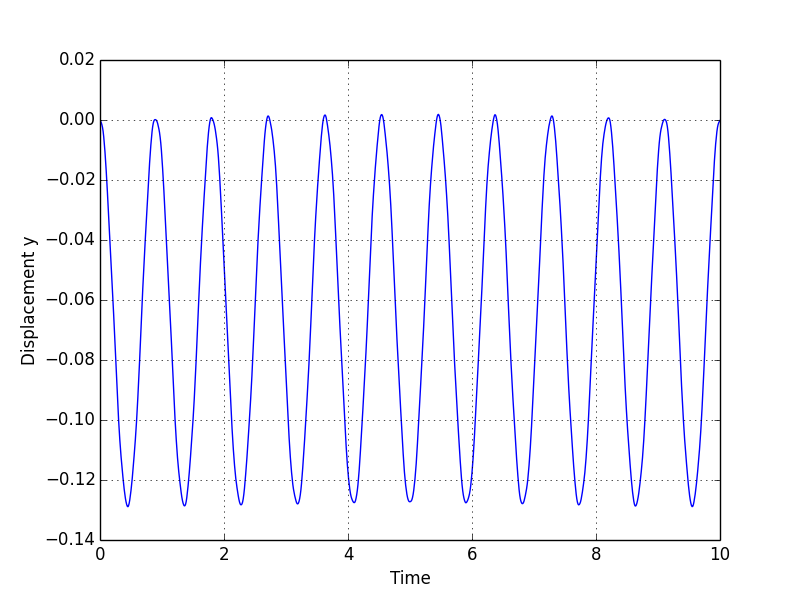
\includegraphics[width=0.9\linewidth,trim={2mm 2mm 5mm 5mm},clip]{./Verification_Validation//Hron_Turek/dis_y.png} 
    \caption{Displacement in x direction, timeinterval (0,10)} 
    \vspace{4ex}
  \end{minipage} 
  \begin{minipage}[b]{0.60\linewidth}
    \centering
    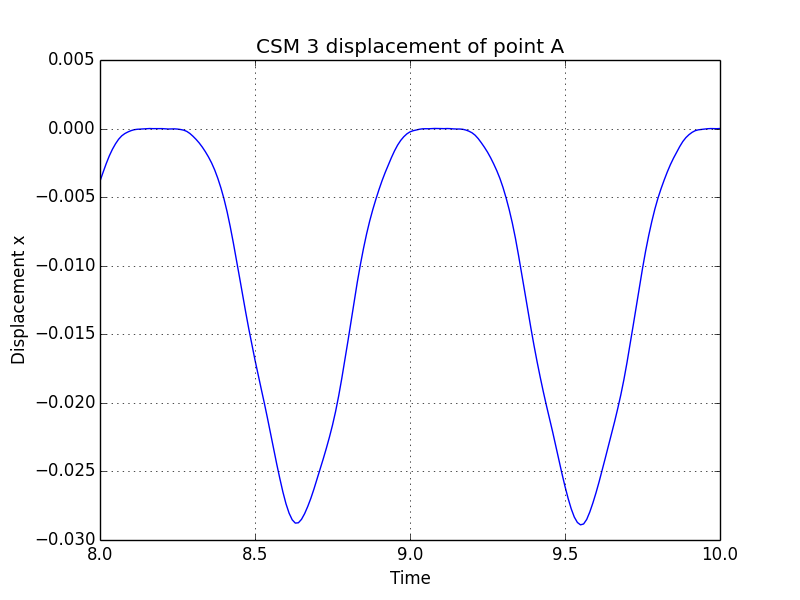
\includegraphics[width=0.9\linewidth,trim={2mm 2mm 5mm 5mm},clip]{./Verification_Validation//Hron_Turek/dis_x_short.png} 
    \caption{Displacement in x direction, timeinterval (8,10)} 
    \vspace{4ex}
  \end{minipage}%% 
  \begin{minipage}[b]{0.60\linewidth}
    \centering
    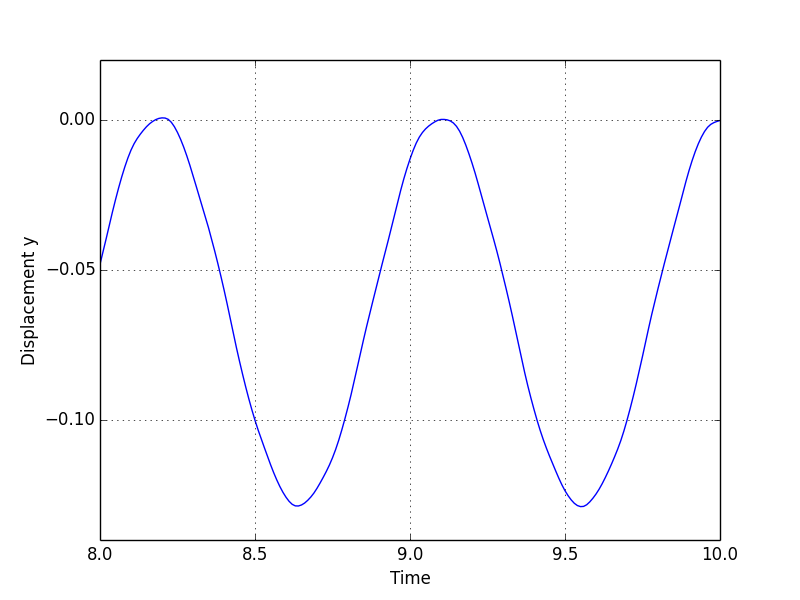
\includegraphics[width=0.9\linewidth,trim={2mm 2mm 5mm 5mm},clip]{./Verification_Validation/Hron_Turek/dis_y_short.png} 
    \caption{Displacement in x direction, timeinterval (8,10)} 
    \vspace{4ex}
  \end{minipage} 
\end{figure}

\subsubsection*{Discussion of the CSM results}
The tables \ref{tab:CSM1}, \ref{tab:CSM2} shows the results of the two steady state cases with different bar-stiffness. As the number of spatial points in the domain increases the solutions converge towards the referential value. The CSM3 case shown in table \ref{tab:CSM3} shows the same trend of converging toward referential value when the number of spatial points are increased.

The plot \ref{plot:CSM3_plots} is of displacement at the point A in x and y direction of the CSM3 test. The CSM3 test was run with Crank-Nicholson, $\theta = 0.5$, and it can be seen that in the y displacement the bar returns to it initial state, that is with zero displacement. This results indicates that the energy in the system has been preserved.

\subsubsection*{FSI tests}
Lastly the full FSI problem ran. Here we can see in \ref{fig:fluid_structure} that now both fluid and structure has a mesh. The tests are run with 2 different inflows conditions. FSI1 gives a steady state solution while the others are unsteady. FSI-2 gives the largest deformation is therefore considered the most difficult of the three \cite{Richter2013}, giving deformations of 2.5 times greater than the flag height. Vinje 2016 \cite{Vinje2016} reported not being able to compute FSI-2 model due to shortcomings in the linear elasticity solid model. The FSI-3 test has the highest inflow speed giving medium deformations but more rapid oscillations.

\begin{figure}[H]
\label{fig:fluid_structure}
\caption{Fluid and Structure computing mesh}
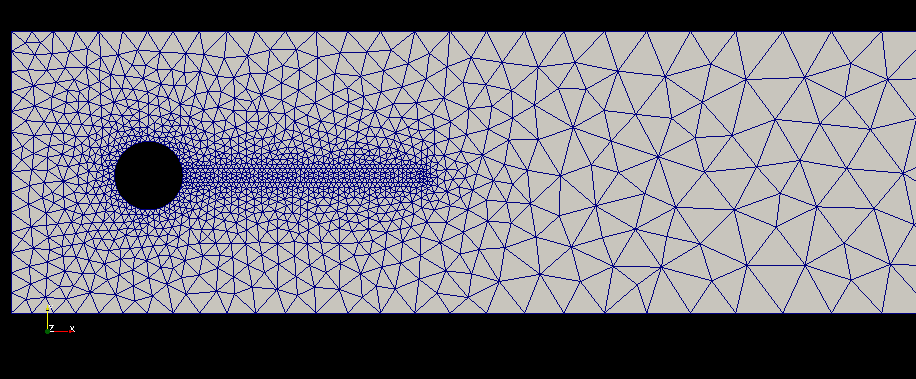
\includegraphics[scale=0.45, trim={4mm 21mm 2mm 10mm},clip]{./Verification_Validation/Hron_Turek/fluid_structure.png}
\end{figure}

\begin{table}[h!]
\centering
\caption{FSI Parameters}
\label{my-label}
\begin{tabular}{|l|l|l|l|}
\hline
Parameters & FSI1 & FSI2 & FSI3 \\ \hline
$\rho_f[10^3 \frac{kg}{m^3}]$ & 1 & 1 & 1 \\ \hline
$\nu_f [10^{-3} \frac{m^2}{s}]$ & 1 & 1 & 1 \\ \hline
$u_0$ & 0.2 & 1 & 2 \\ \hline
Re = $\frac{U d}{\nu_f}$ & 20 & 100 & 200 \\ \hline
$\rho_s[10^3 \frac{kg}{m^3}]$ & 1 & 10 & 1 \\ \hline
$\nu_s$ & 0.4 & 0.4 & 0.4 \\ \hline
$\mu_s[10^6 \frac{m^2}{s}]$ & 0.5 & 0.5 & 2 \\ \hline
\end{tabular}
\end{table}

\subsubsection*{FSI1}
\begin{table}[H]
\centering
\caption{FSI 1}
\label{my-label}
\begin{tabular}{|l|l|l|l|l|l|l|}
\hline
Cells & Dofs & $d_x(A) [\times10^{-3}]$ & $d_y(A)[\times10^{-3}]$ & Drag & Lift & Spaces \\ \hline
2698 & 23563 &0.0227418 &0.799314  &  14.1735 &0.761849 & P2-P2-P1 \\ \hline
10792 & 92992  &0.0227592 & 0.80795 & 14.1853 &  0.775063 &  P2-P2-P1 \\ \hline
43168 & 369448 & 0.0227566 & 0.813184 & 14.2269 & 0.771071 & P2-P2-P1 \\ \hline
\textbf{ref} & \textbf{ref} & \textbf{0.0227} & \textbf{0.8209} & \textbf{14.295} & \textbf{0.7638} & \textbf{ref} \\ \hline
\end{tabular}
\end{table}

\subsubsection*{FSI2}

\begin{comment}
\begin{table}[H]
\centering
\caption{FSI-2 with $\Delta t = 0.01$}
\label{my-label}
\begin{tabular}{|l|l|l|l|l|l|l|l|l|}
\hline
Cells & Dofs & $d_x(A) [\times 10^{-3}]$ & $d_y(A) [\times10^{-3}]$ & Drag & Lift & Extrapolation & BC & $\Delta t$ \\ \hline
2698 & 23563 & $-15.17 \pm 13.35  $ & $1.13 \pm 82.5$ & $160.12 \pm 17.88$ & $0.87 \pm 259.62$ & Biharmonic & 1 & 0.01 \\ \hline
2698 & 23563 & $-14.92 \pm 13.17 $ & $1.13 \pm 81.86$ & $160.28 \pm 17.94$ & $0.65 \pm 254.07$ & Biharmonic & 2 & 0.01 \\ \hline
2698 & 23563 & $-15.10 \pm 13.32 $ & $1.16 \pm 82.46 $ & $159.53 \pm,17.44 $ & $ 0.68 \pm 259.10 $ & Harmonic & - & 0.01 \\ \hline
10792 & 92992 & $-14.83 \pm 13.11 $ & $1.24 \pm 81.72$ & $ 161.50 \pm 18.17  $ & $0.89 \pm 255.10 $ & Harmonic & - & 0.01 \\ \hline
\textbf{ref} & \textbf{ref} & $\textbf{-14.58} \pm \textbf{12.44}$ & $\textbf{1.23} \pm \textbf{80.6}$ & $\textbf{208.83} \pm \textbf{73.75}  $ & $\textbf{0.88} \pm \textbf{234.2} $ & \textbf{ref} & \textbf{ref} & \textbf{ref} \\ \hline
\end{tabular}
\end{table}
\end{comment}


\begin{table}[H]
\centering
\caption{FSI-2 with $\Delta t = 0.01$ harmonic}
\label{my-label}
\begin{tabular}{|l|l|l|l|l|l|}
\hline
Cells & Dofs & $d_x(A) [x10^{-3}]$ & $d_y(A) [x10^{-3}]$ & Drag & Lift \\ \hline
2698 & 23563 & $ -15.10 \pm 13.32 $ & $1.16 \pm 82.46 $ & $ 159.53 \pm 17.44 $ & $ 0.68 \pm 259.10 $ \\ \hline
10792 & 92992 & $ -14.85 \pm 13.14 $ & $1.21 \pm 81.72 $ & $ 160.72 \pm 17.84  $ & $0.93 \pm 255.14 $ \\ \hline
43168 & 369448 & $ -14.83  \pm 13.11  $ & $ 1.24 \pm 81.6 $ & $ 161.50 \pm 18.17  $ & $0.62 \pm 254.40  $ \\ \hline
\textbf{ref} & \textbf{ref} & $\textbf{-14.58} \pm \textbf{12.44}$ & $\textbf{1.23} \pm \textbf{80.6}$ & $\textbf{208.83} \pm \textbf{73.75}  $ & $\textbf{0.88} \pm \textbf{234.2} $ \\ \hline
\end{tabular}
\end{table}

\begin{table}[H]
\centering
\caption{FSI-2 with $\Delta t = 0.001$}
\label{my-label}
\begin{tabular}{|l|l|l|l|l|l|l|}
\hline
Cells & Dofs & $d_x(A) [\times10^{-3}]$ & $d_y(A) [\times10^{-3}]$ & Drag & Lift  \\ \hline
2698 & 23563 & $ 15.42 \pm 13.10$ & $1.14 \pm 83.39$ & $157.01 \pm 15.69$ & $ -0.77 \pm 274.36$  \\ \hline
10792 & 92992 & $ 15.16 \pm 12.94$ & $ 1.20 \pm 82.5 $ & $ 158.26 \pm 16.03$ & $ -0.09 \pm 267.81$  \\ \hline
\textbf{ref} & \textbf{ref} & $\textbf{-14.58} \pm \textbf{12.44}$ & $\textbf{1.23} \pm \textbf{80.6}$ & $\textbf{208.83} \pm \textbf{73.75}  $ & $\textbf{0.88} \pm \textbf{234.2} $ \\ \hline
\end{tabular}
\end{table}

\begin{figure}[H]
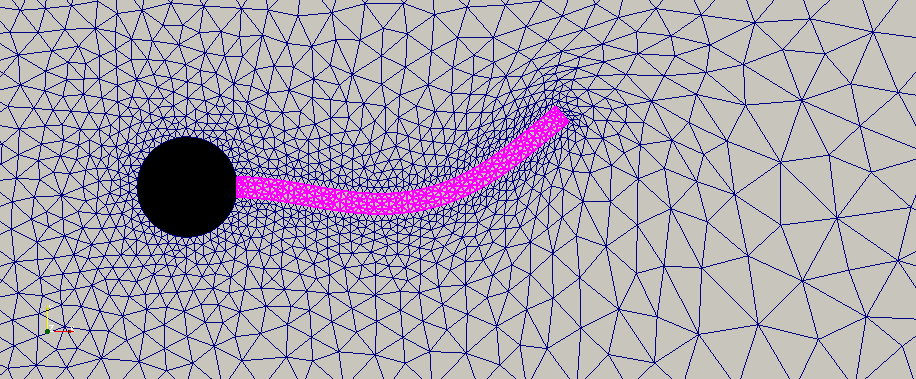
\includegraphics[scale=0.40,trim={0mm 0mm 0mm 0mm},clip]{./Verification_Validation/Hron_Turek/FSI2_d_920.png}
\caption{Deformation at $t =9.20 $sec. The bar is marked with pink colour and deformed using warp by vector in paraview.}
\end{figure}
\begin{figure}[H]
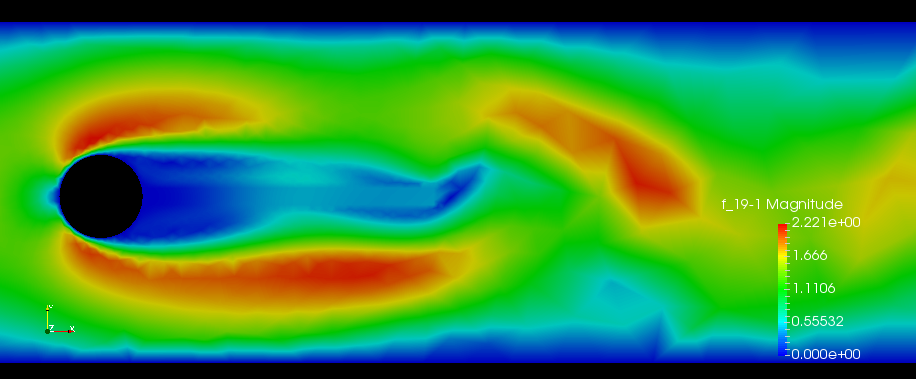
\includegraphics[scale=0.40,trim={0mm 0mm 0mm 0mm},clip]{./Verification_Validation/Hron_Turek/FSI2_u_920.png}
\caption{Fluid velocity at $ t = 9.20 $sec on the reference mesh}
\end{figure}

\subsubsection*{FSI3}
\begin{table}[H]
\centering
\caption{FSI3 with $\Delta t = 0.01$}
\label{my-label}
\begin{tabular}{|l|l|l|l|l|l|}
\hline
 &  & $d_x(A) [\times10^{-3}]$ & \& $d_y(A)[\times10^{-3}]$ & Lift & Drag \\ \hline
0 & bi\_bc2 & $-1.74 \pm 1.766$ & $ 3.565e \pm 26.01 $ & $ -1.357 \pm 138.74$ & $439.41 \pm12.218$ \\ \hline
 & bi\_bc1 & $-1.77 \pm 1.793$ & $ 3.582 \pm 26.21 $ & $ -1.843 \pm 139.29$ & $439.60\pm12.218$ \\ \hline
 & laplace & $-1.791 \pm 1.807$ & $ 3.290 \pm 26.48 $ & $1.960 \pm 142.306$ & $ 439.35 \pm 12.04$ \\ \hline
 &  &  &  &  &  \\ \hline
1 & bi\_bc2 & $-2.397 \pm 2.406$ & $ 1.774 \pm 32.282 $ & $ 3.668 \pm 150.02$ & $ 449.71 \pm 18.172$ \\ \hline
 & bi\_bc1 & $ -2.440 \pm 2.446$ & $ 1.766 \pm 32.562 $ & $ 3.929 \pm 150.76$ & $ 449.98 \pm 18.030$ \\ \hline
 & laplace & $ -2.481 \pm 2.486$ & $ 1.655 \pm 32.851$ & $ 3.318 \pm 153.58$ & $ 449.74 \pm18.052$ \\ \hline
ref. &  & $ ?2.69 \pm 2.53$ & $1.48 \pm 34.38 $ & $ 2.22 \pm 149.78$ & $ 457.3 \pm 22.66$ \\ \hline
\end{tabular}
\end{table}

\subsection*{Comment on FSI tests}
The FSI1 test gives a low fluid velocity and gives very low displacements. FSI1 is therefore not a rigid test for FSI. In fact I experienced in the beginning of making the FSI solver, that even with a wrong implementation i got good FSI1 results. However it is a good test for early checks, because if FSI1 is wrong the rest will definitely not work.  \newline

FSI2 has a Reynolds number of 100 with medium fluid speeds. It does however induce great deformations and is therefore a great FSI test. Using a mesh motion technique that upholds the mesh structure is crucial. The results shown are with the Harmonic extension but I got similar results for biharmonic extension. The FSI2 test could be run with a fairly large time $\Delta t = 0.01 $, since the fluid velocity is not very high. And it can been seen from the results that choosing a time step $\Delta t = 0.001$ did not yield much better results. The Drag was computed to be about a value of 40 less than reported by Hron and Turek. This i believe is because a combination of the way the mesh was constructed, without a good enough boundary layer, and the mapping to a reference configuration. +++ \newline

Lastly the FSI3 test has a Reynolds number of 200 with greater inflow speeds. The run time improvements such as reusing the jacobian did not work with the FSI3 test. The Jacobian needed to be more precise than for FSI2. For this reason a different mesh, with lower number of cells needed to be used in FSI3.  +++

















